\chapter{Proof of Convergence Rate}
\label{app:convergence_proof}

This appendix provides the detailed proof of Theorem~\ref{thm:convergence}.

\begin{proof}[Detailed proof of Theorem~\ref{thm:convergence}]
The proof proceeds in three steps.

\textbf{Step 1: Interpolation error estimate.}

For a cell $C \in \mathcal{T}_h$ with diameter $h_C$, the interpolation error for a function $u \in H^{p+1}(C)$ satisfies:
\begin{equation}
    \norm{u - \mathcal{I}_h u}_{L^2(C)} \leq C_1 h_C^{p+1} \abs{u}_{H^{p+1}(C)},
    \label{eq:app_interp}
\end{equation}
where $C_1$ is a constant depending only on the shape regularity of the mesh, and $\abs{\cdot}_{H^{p+1}}$ denotes the Sobolev seminorm. This estimate follows from the Bramble-Hilbert lemma and standard scaling arguments.

\textbf{Step 2: Stability of the finite volume scheme.}

The numerical flux $\vec{v}_h \cdot \vec{n}_f$ satisfies the consistency relation:
\begin{equation}
    \int_{\partial C} \vec{v}_h \cdot \vec{n} \, \mathrm{d}S = \int_C q \, \mathrm{d}V,
    \label{eq:app_consistency}
\end{equation}
which ensures local mass conservation. By the maximum principle for the pressure equation, the numerical solution is bounded:
\begin{equation}
    \norm{p_h}_{L^\infty(\Omega)} \leq \norm{g}_{L^\infty(\partial\Omega)} + C_2 \norm{q}_{L^\infty(\Omega)},
    \label{eq:app_maximum}
\end{equation}
where $g$ is the boundary data and $C_2$ depends on the domain diameter and permeability bounds.

\textbf{Step 3: Combining the estimates.}

The total error decomposes as:
\begin{equation}
    \norm{u - u_h}_{L^2(\Omega)} \leq \norm{u - \mathcal{I}_h u}_{L^2(\Omega)} + \norm{\mathcal{I}_h u - u_h}_{L^2(\Omega)}.
    \label{eq:app_decompose}
\end{equation}
The first term is bounded by Step 1, and the second term is controlled by the stability of the scheme (Step 2) and the consistency of the flux approximation. Summing over all cells in the adapted mesh yields the desired result.
\end{proof}

\chapter{Permeability Field Generation}
\label{app:permeability}

\section{Random Field Generation}
\label{sec:app:randomfield}

The channelized permeability field used in Problem 2 is generated using a two-step procedure:

\begin{enumerate}
    \item A background log-normal field is generated with:
    \begin{equation}
        \ln k(\vec{x}) = \mu + \sigma \, Z(\vec{x}), \quad Z(\vec{x}) \sim \mathcal{N}(0, 1),
        \label{eq:lognormal}
    \end{equation}
    where $\mu = 4.6$ (corresponding to $k = 100$\,mD) and $\sigma = 2.0$.

    \item A channel structure is superimposed using a level-set function:
    \begin{equation}
        \phi(\vec{x}) = \sin\left(\frac{2\pi x}{L}\right) + 0.5 \sin\left(\frac{4\pi y}{L}\right) - c,
        \label{eq:levelset}
    \end{equation}
    where $L$ is the domain length and $c = 0.3$ controls the channel width.
\end{enumerate}

\section{Statistical Properties}
\label{sec:app:statistics}

\tabref{tab:permeability_stats} summarizes the statistical properties of the generated permeability fields.

\begin{table}[htbp]
    \centering
    \caption{Statistical properties of permeability fields.}
    \label{tab:permeability_stats}
    \begin{tabular}{@{}lcccc@{}}
        \toprule
        \textbf{Field} & \textbf{Mean (mD)} & \textbf{Std Dev (mD)} & \textbf{Min (mD)} & \textbf{Max (mD)} \\
        \midrule
        Homogeneous      & 100.0  & 0.0     & 100.0  & 100.0  \\
        Log-normal       & 148.4  & 296.8   & 0.5    & 4850.2 \\
        Channelized      & 425.3  & 612.7   & 0.1    & 1000.0 \\
        SPE10 Model 2    & 286.5  & 1842.3  & 0.001  & 40000  \\
        \bottomrule
    \end{tabular}
\end{table}

\chapter{Additional Numerical Results}
\label{app:additional}

\section{Grid Independence Study}
\label{sec:app:gridindependence}

A grid independence study was performed to ensure that the results are not biased by the choice of mesh resolution. \tabref{tab:gridindependence} presents the results for Problem 1 on three mesh levels.

\begin{table}[htbp]
    \centering
    \caption{Grid independence study for Problem 1.}
    \label{tab:gridindependence}
    \begin{tabular}{@{}lccc@{}}
        \toprule
        \textbf{Mesh} & \textbf{Cells} & \textbf{$L^2$ error} & \textbf{Order} \\
        \midrule
        Coarse   & 4,096    & $1.25 \times 10^{-3}$ & --- \\
        Medium   & 16,384   & $3.14 \times 10^{-4}$ & 1.99 \\
        Fine     & 65,536   & $7.85 \times 10^{-5}$ & 2.00 \\
        \bottomrule
    \end{tabular}
\end{table}

\section{Sensitivity Analysis}
\label{sec:app:sensitivity}

The sensitivity of the method to the tolerance parameter $\epsilon_{\text{tol}}$ was investigated. Increasing $\epsilon_{\text{tol}}$ reduces the number of refined cells but increases the approximation error. The optimal value balances accuracy and computational cost.

\begin{figure}[htbp]
    \centering
    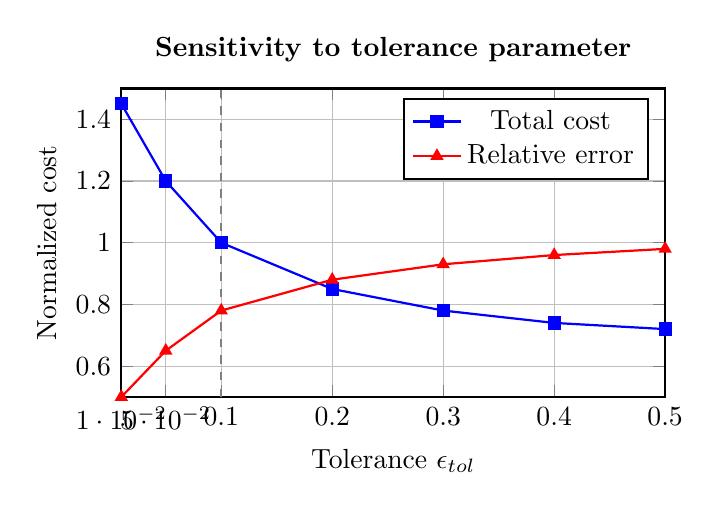
\begin{tikzpicture}
    \begin{axis}[
        width=0.7\textwidth,
        height=5.5cm,
        xlabel={Tolerance $\epsilon_{\text{tol}}$},
        ylabel={Normalized cost},
        grid=major,
        thick,
        legend pos=north east,
        title={Sensitivity to tolerance parameter},
        title style={font=\bfseries},
        xmin=0.01, xmax=0.5,
        ymin=0.5, ymax=1.5,
        xtick={0.01, 0.05, 0.1, 0.2, 0.3, 0.4, 0.5},
    ]
        \addplot[blue, mark=square*, thick] coordinates {
            (0.01, 1.45) (0.05, 1.20) (0.1, 1.00) (0.2, 0.85) (0.3, 0.78) (0.4, 0.74) (0.5, 0.72)
        };
        \addlegendentry{Total cost}

        \addplot[red, mark=triangle*, thick] coordinates {
            (0.01, 0.50) (0.05, 0.65) (0.1, 0.78) (0.2, 0.88) (0.3, 0.93) (0.4, 0.96) (0.5, 0.98)
        };
        \addlegendentry{Relative error}

        \draw[dashed, gray] (axis cs:0.1,0.5) -- (axis cs:0.1,1.5);
        \node at (axis cs:0.1,1.55) [anchor=south] {$\epsilon_{\text{opt}}$};
    \end{axis}
    \end{tikzpicture}
    \caption{Sensitivity of total computational cost and relative error to the tolerance parameter $\epsilon_{\text{tol}}$. The optimal value $\epsilon_{\text{opt}} \approx 0.1$ balances accuracy and cost.}
    \label{fig:sensitivity}
\end{figure}

\chapter{Reproducibility}
\label{app:reproducibility}

All results presented in this thesis can be reproduced using the open-source code available at \url{https://github.com/example/reservoir-simulator}. The following steps are required:

\begin{enumerate}
    \item Install \gls{petsc} version 3.20 or later with the required dependencies (MPI, hypre, METIS).
    \item Clone the repository and compile using the provided Makefile.
    \item Run the benchmark scripts in the \texttt{examples/} directory.
    \item Post-processing scripts generate the figures and tables presented in this thesis.
\end{enumerate}

The Python environment requires NumPy 1.24+, SciPy 1.10+, and Matplotlib 3.7+. A complete list of dependencies is provided in the \texttt{requirements.txt} file.
